\section{Field density vs node/edge usage}
\label{sec:field_density_usage}
\noindent\textit{Analysis \texttt{field\_density\_usage}, 38 sessions, fingerprint \texttt{54f6a1984e6f}.}

7{,}483 element$\times$session observations (37 sessions; elements with $>50\%$ valid bins and at least one visit). The within-session Spearman correlation between field density and visits was -0.23 (median; positive in 0 of 37 sessions); for spike-shift surrogates of the same cells it was -0.63.

In the Poisson GLM the slope of field count on $\ln$(visits) is $-0.19 \pm 0.01$ for the observed fields and $-0.36 \pm 0.01$ for the surrogates (Table~\ref{tab:field_density_usage:glm}). The surrogate slope is the steeper of the two: rarely visited elements have noisier rate estimates and therefore more spurious peaks, so the negative relation is expected from the detector alone. With the element's surrogate density as a covariate the observed slope is $-0.05 \pm 0.01$. Relative to that noise floor, fields are thus not depleted in heavily used elements.

\begin{table}[htbp]
\centering
\small
\caption{Maze elements entering the analysis (summed over sessions).}
\label{tab:field_density_usage:elements}
\begin{tabular}{lrrrrrr}
\toprule
kind & observations & median visits & median occupancy (s) & field peaks & track (m) & peaks / m \\
\midrule
edge & 4{,}120 & 4 & 2.99 & 18{,}639 & 1102 & 16.9 \\
node & 3{,}363 & 4 & 3.09 & 4{,}928 & 538 & 9.16 \\
\bottomrule
\end{tabular}
\end{table}
\begin{table}[htbp]
\centering
\footnotesize
\caption{Poisson GLM, \texttt{n\_peaks $\sim$ usage + kind + session}, offset $\ln$(length), session-clustered standard errors. A usage coefficient of 1 means field count is proportional to usage; 0 means no dependence. \emph{surrogate}: the same model on spike-shift surrogate fields (detector bias only). \emph{observed | surrogate}: observed peaks with the element's surrogate density as an additional covariate.}
\label{tab:field_density_usage:glm}
\begin{tabular}{llllrrrr}
\toprule
usage & group & data & term & coef & se & z & p \\
\midrule
ln visits & pooled & observed & usage & -0.194 & 0.0122 & -15.9 & $7.75\times10^{-57}$ \\
ln visits & pooled & surrogate & usage & -0.364 & 0.00937 & -38.8 & 0 \\
ln visits & pooled & observed | surrogate & usage & -0.0509 & 0.0135 & -3.78 & $1.58\times10^{-4}$ \\
ln visits & pooled & observed | surrogate & ln surrogate density & 0.388 & 0.0281 & 13.8 & $1.92\times10^{-43}$ \\
ln visits & Rat5 & observed & usage & -0.193 & 0.0246 & -7.85 & $4.10\times10^{-15}$ \\
ln visits & Rat5 & surrogate & usage & -0.361 & 0.00854 & -42.3 & 0 \\
ln visits & Rat5 & observed | surrogate & usage & -0.0671 & 0.0217 & -3.08 & 0.00205 \\
ln visits & Rat5 & observed | surrogate & ln surrogate density & 0.353 & 0.041 & 8.63 & $6.10\times10^{-18}$ \\
ln visits & Rat6 & observed & usage & -0.194 & 0.0137 & -14.2 & $8.99\times10^{-46}$ \\
ln visits & Rat6 & surrogate & usage & -0.365 & 0.0143 & -25.6 & $4.06\times10^{-144}$ \\
ln visits & Rat6 & observed | surrogate & usage & -0.04 & 0.0174 & -2.29 & 0.0219 \\
ln visits & Rat6 & observed | surrogate & ln surrogate density & 0.412 & 0.0385 & 10.7 & $8.95\times10^{-27}$ \\
ln occupancy & pooled & observed & usage & -0.194 & 0.00959 & -20.2 & $3.72\times10^{-91}$ \\
ln occupancy & pooled & surrogate & usage & -0.259 & 0.00808 & -32.1 & $3.59\times10^{-226}$ \\
ln occupancy & pooled & observed | surrogate & usage & -0.115 & 0.00984 & -11.7 & $1.52\times10^{-31}$ \\
ln occupancy & pooled & observed | surrogate & ln surrogate density & 0.305 & 0.0257 & 11.9 & $1.39\times10^{-32}$ \\
ln occupancy & Rat5 & observed & usage & -0.183 & 0.0163 & -11.3 & $1.60\times10^{-29}$ \\
ln occupancy & Rat5 & surrogate & usage & -0.245 & 0.00721 & -34 & $1.16\times10^{-253}$ \\
ln occupancy & Rat5 & observed | surrogate & usage & -0.114 & 0.0131 & -8.67 & $4.51\times10^{-18}$ \\
ln occupancy & Rat5 & observed | surrogate & ln surrogate density & 0.29 & 0.0375 & 7.75 & $9.13\times10^{-15}$ \\
ln occupancy & Rat6 & observed & usage & -0.201 & 0.0121 & -16.6 & $5.07\times10^{-62}$ \\
ln occupancy & Rat6 & surrogate & usage & -0.269 & 0.0123 & -21.9 & $1.63\times10^{-106}$ \\
ln occupancy & Rat6 & observed | surrogate & usage & -0.116 & 0.0141 & -8.21 & $2.14\times10^{-16}$ \\
ln occupancy & Rat6 & observed | surrogate & ln surrogate density & 0.313 & 0.035 & 8.92 & $4.62\times10^{-19}$ \\
\bottomrule
\end{tabular}
\end{table}
\begin{table}[htbp]
\centering
\footnotesize
\caption{Slope on $\ln$(visits) when only elements with at least \texttt{min\_visits} visits are kept.}
\label{tab:field_density_usage:robust}
\begin{tabular}{rrlrrrr}
\toprule
min.\ visits & observations & data & coef & se & z & p \\
\midrule
1 & 7{,}483 & observed & -0.194 & 0.0122 & -15.9 & $7.75\times10^{-57}$ \\
1 & 7{,}483 & surrogate & -0.364 & 0.00937 & -38.8 & 0 \\
3 & 5{,}558 & observed & -0.183 & 0.0172 & -10.6 & $1.95\times10^{-26}$ \\
3 & 5{,}558 & surrogate & -0.478 & 0.0143 & -33.3 & $5.77\times10^{-243}$ \\
5 & 3{,}520 & observed & -0.128 & 0.0269 & -4.76 & $1.93\times10^{-6}$ \\
5 & 3{,}520 & surrogate & -0.518 & 0.0194 & -26.7 & $1.33\times10^{-157}$ \\
10 & 1{,}127 & observed & -0.0155 & 0.0842 & -0.184 & 0.854 \\
10 & 1{,}127 & surrogate & -0.595 & 0.0575 & -10.4 & $4.07\times10^{-25}$ \\
\bottomrule
\end{tabular}
\end{table}

\begin{figure}[htbp]
\centering
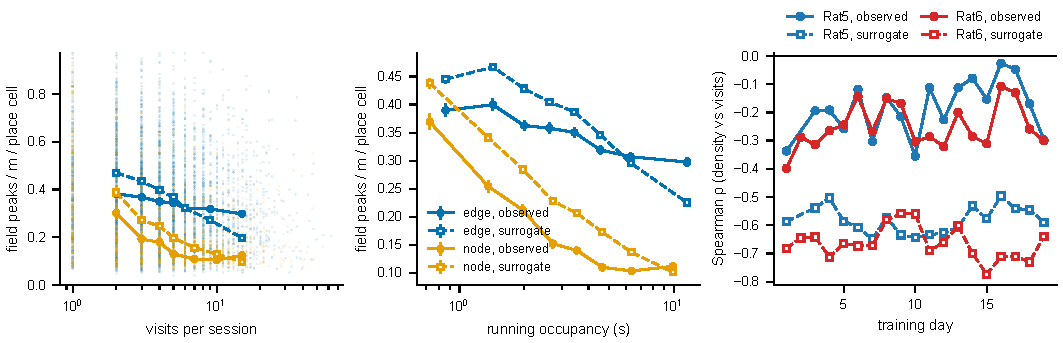
\includegraphics[width=\textwidth]{field_density_usage__field_density_usage.pdf}
\caption{\textbf{Field density vs usage.} Left: field peaks per metre per place cell against the number of visits; dots are single maze elements in single sessions, markers are means $\pm$ s.e.m.\ in visit octiles. Filled/solid: observed. Open/dashed: spike-shift surrogates of the same cells (spatial tuning destroyed, rate and maze sampling preserved). Middle: the same against running occupancy. Right: within-session Spearman correlation between field density and visits, per training day.}
\label{fig:field_density_usage}
\end{figure}

\clearpage